\section{Análisis}

En esta sección presentaremos el análisis de los distintos casos de estudio abordados. Cada subsección corresponderá a uno de ellos, abordándolos de menor a mayor tamaño.

\subsection{Red doméstica}

% \indent \indent En este caso estudiamos la red de una oficina con alrededor de 40 computadoras y teléfonos celulares.\\
% \indent La captura duró alrededor de seis horas y se compone de más de noventa mil mensajes ARP who-has. Con este volumen de datos fue necesario seccionar el análisis bajo diferentes criterios a la hora de observar los grafos dirigidos que se crearon en base a los resultados, como la cantidad de mensajes o una cantidad mínima de mensajes entre nodos.\\

% \subsubsection{Detección de nodos significativos}

% %Nos interesa poder detectar de manera automática nodos significativos midiendo la \textit{información} contra la \textit{entropía} de la fuente como explicamos en la sección \textit{desarrollo}.\newline

% \indent \indent Siguiendo el método indicado en la sección \textbf{Desarrollo}, calculamos la entropía de las fuentes y la información de los símbolos de cada una, para poder contrastarlos.\\
% \indent Con los datos obtenidos, se confeccionaron los siguientes gráficos:\\

% \begin{center}
% \includegraphics[scale=0.5,clip=true,trim=100 0 0 0]{graphics/tonchis_src.png}

% \includegraphics[scale=0.5,clip=true,trim=100 0 0 0]{graphics/tonchis_dst.png}
% \end{center}

% \indent Más en detalle, los datos de los nodos que consideramos distinguidos de acuerdo al criterio establecido son:\\
% \begin{center}
% \begin{tabular}{c c}
% \begin{tabular}{ | c | c  | }
% 	\hline
% 	Entropía origen & 3.44 bits\\
% 	\hline
% 	IP                      & Información \\
% 	\hline
% 	192.168.0.1     & 1.41 bits\\
% 	0.0.0.0 		     & 3.21 bits\\
% 	\hline
% \end{tabular}
% &
% \begin{tabular}{ | c | c  | }
% 	\hline
% 	Entropía destino & 4.65 bits\\
% 	\hline
% 	IP 		                  & Información \\
% 	\hline
% 	192.168.0.193  & 2.09 bits\\
% 	192.168.0.1      & 2.48 bits\\
% 	192.168.0.195  & 3.00 bits\\
% 	\hline
% \end{tabular}
% \end{tabular}
% \end{center}


% \subsubsection{Grafos de la captura}

% \indent \indent Antes de analizar la captura sosteníamos como hipótesis que la topología de los mensajes ``tendría forma de árbol'' con el router en su raíz y tantas hojas como hosts dentro de la red, con poco o nada de interacción entre ellos.\\
% \indent También suponíamos que la mayoría de las redes \textit{subneteadas} con un router tendrían necesariamente esta forma.\\
% \indent Los grafos presentados a continuación muestran direcciones IP como nodos unidos por un eje si el nodo origen realizó un broadcast ARP who-has buscando al nodo destino (en este experimento, el peso de estos ejes representa la cantidad de mensajes enviados).\\
% \indent Para empezar, mostramos los primeros diez mil requests entre los nodos que se enviaron diez o más mensajes. Elegimos esta parte de la muestra tras haber visto que graficar más nodos agrega poca información nueva respecto de los nodos más relevantes.\\

% \begin{center}
% \includegraphics[scale=0.25,angle=90]{graphics/t-work-10000c-10w.png}
% \end{center}

% \indent A primera vista notamos que hay ciertos nodos que resaltan sobre los demás como el 192.168.0.1 (router), o 192.168.0.126. Si bien la estructura de este digrafo no es un árbol, se nota que hay cierta jerarquía. En particular, se puede observar la relevancia del nodo 192.168.0.1, uno de los que en base a nuestro criterio consideramos como distinguido.\\
% \indent Un nodo interesante que resalta es el 169.254.255.255, porque es la única IP no privada que aparece en la red. Analizando este caso en particular, vemos que siempre es buscado por nodos de la red (y éste nunca busca a nadie), lo que nos hace suponer que puede tratarse de un servicio, como un servidor de DNS. Sin embargo, no es lo suficientemente relevante para ser considerado un nodo distinguido siguiendo nuestro criterio:\\

% \includegraphics[scale=0.25,clip=true,trim=700 0 720 0]{graphics/t-work-ip-169-254-255-255.png}

% \indent Investigando el resto de la captura, notamos que los demás paquetes que recibe son del protocolo NetBIOS Name Service, con lo que podemos afirmar que en este nodo funciona un NetBIOS Server.\\
% \indent Para poder verificar mejor si los nodos distinguidos del inciso anterior se corresponden con los nodos más importantes de la red veamos el siguiente grafo, donde se estudia toda la muestra pero sólo nos quedamos con aquellos nodos que compartieron más de mil mensajes.\newline

% \includegraphics[scale=0.30]{graphics/t-work-all-1000w.png}

% \indent Y un poco más en detalle, enfocándonos en el router, es decir en la dirección 192.168.0.1:\\

% \begin{center}
% \includegraphics[scale=0.3]{graphics/t-work-router-1000w.png}
% \end{center}

% \indent Viendo los mensajes ARP de esta manera en ambos grafos podemos notar varias cosas. Por un lado que tiene forma de árbol, pero el nodo raíz no es el router, como suponíamos originalmente. Vemos que en concordancia con nuestra consideración de nodo distinguido para la fuente origen, hay muchos requests ARP que tienen origen en el 0.0.0.0 y como destino diversos nodos de la red, aunque ésta no es una IP del rango privado.\\
% \indent Este nos llevó a investigar y conocer que un ARP con origen 0.0.0.0 es parte de una técnica para detectar direcciones IP duplicadas dentro de una red. En este caso, se estaba queriendo detectar si las direcciones terminadas en 51, 56, 68, 76 ó 164 estaban duplicadas.\\
% \indent Es notable la gran cantidad de pedidos que recibe la IP 192.168.0.195, otro de los nodos que distinguimos con nuestro criterio.\\
% \indent De estos grafos se extrae además que dos de los nodos que consideramos distinguidos son los que más \textit{request ARP} intercambian, ocurriendo que  192.168.0.1 busca a 192.168.0.193 21301 veces. Estos gráficos parecen confirmar la efectividad del criterio (distinguir aquellos nodos cuya información contenida es menor a la entropía de la fuente), puesto que nos permite establecer la correspondencia del nodo 192.168.0.1 como  distinguido para la fuente origen, y el 192.168.0.193 como distinguido para la fuente destino.\\
% \indent El grafo enfocado en el router nos permite además verificar que en efecto la dirección 192.168.0.1 es un nodo distinguido para la fuente destino.\\
% \indent Nos resultó interesante la gran cantidad de veces que se pide la IP 192.168.0.193 y el porqué de que podamos considerarlo un nodo distinguido. Para saber más sobre lo que podría estar sucediendo con ese host, revisamos el resto de la captura pero encontramos que no había ningún paquete con esa dirección origen ni destino.\\
% \indent Por esto creemos que podría tratarse de un nodo mal configurado, buscando el router una IP que ya no existe en la red, lo cual parece en consonancia con la gran cantidad de pedidos ARP que le hace.\\


\newpage
\subsection{Red Laboral}

En este segundo caso, se analizó una red laboral de una PyME. La captura se realizó por un lapso de media hora en modo promiscuo.

En el gráfico \ref{laboral:graph} se pueden ver los resultados de obtenidos.

\begin{figure}[h!]
    \centering                                                       
    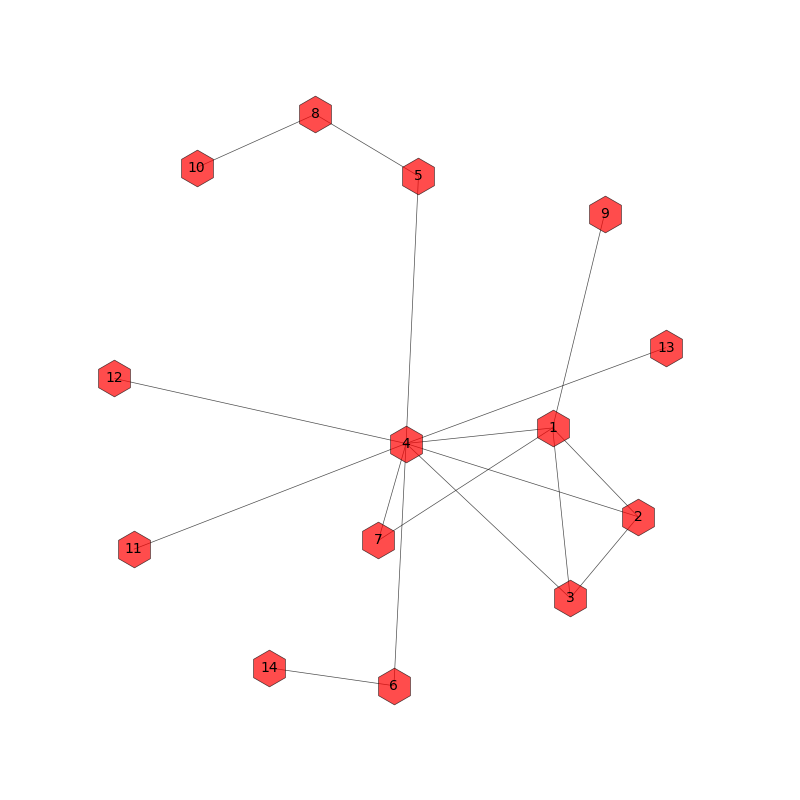
\includegraphics[width=300pt]{img/laboralGraph.png}
    \caption{Grafo de Red Laboral}
    \label{laboral:graph}
\end{figure}

% \indent Dada la enorme cantidad de datos y, además, para analizar un poco la progresión de la captura, se consideraron tres casos.\\
% \indent El primer caso corresponde a los primeros mil paquetes ARP who-has que se capturaron, y nos servirá como primera aproximación. Como caso intermedio, estudiamos luego los primeros seis mil paquetes ARP who-has, que se corresponden aproximadamente con la mitad de los paquetes de dicho tipo capturados a lo largo del experimento. Finalmente, se estudió el caso con todos los paquetes ARP who-has capturados.\\
% \indent En los tres casos se calcularon las entropías de las fuentes \textit{Fuente} y \textit{Destino}, y además se confeccionarion gráficos de barras con la información calculada por IP para las IPs que menos información suministran, que de acuerdo a lo que expresado en la sección \textbf{Desarrollo} son los candidatos a  nodos distinguidos. En tales gŕaficos se puede observar también una recta que representa la entropía de la fuente y que servirá para contrastar visualmente la información de los símbolos con la entropía.\\
% \indent Es oportuno mencionar también que se proveen grafos dirigidos donde el nodo origen corresponde a la IP que pidió a la IP representada por el nodo destino para los primeros dos subcasos de estudio, pero no para el tercero. La sencilla razón es que la gran cantidad de nodos provoca que el grafo sea, a efectos prácticos, ilegible. Estos digrafos los usaremos para confirmar visualmente el estudio realizado.\\
% %\indent Sobre los gŕaficos deseamos hacer un comentario más: si bien los calculamos basados en la cantidad de apariciones de la IP en la correspondiente fuente, es claro que dado lo mencionado en la introducción acerca de que un evento con mayor probabilidad provee menos información, los gráficos que hicimos inducen lo mismo que si en el eje \textit{y} considerásemos el valor numérico de la información de la IP, aunque en ese caso, los histogramas serían \textit{al revés}, en el sentido de que las IP's que aparecen con barras pequeñas en nuestros gráficos lo harían con barras grandes si midiésemos por la infomación que suministra.\\

% \subsubsection{Primeros mil paquetes ARP who-has (Muestra chica)}

% \indent \indent En base a la experimentación realizada, se obtuvieron los siguientes valores de entropía para las fuentes \textit{Fuente} y \textit{Destino}.\\

% \begin{center}
% 	\begin{tabular}{ | c | c | c |} \hline
% 	   & \textbf{$S_{src}$} & \textbf{$S_{dst}$} \\ \hline
% 	  	\textbf{Entropía} & 3,08 bits & 2,75 bits\\ \hline
% 	\end{tabular}
% \end{center}

% \indent \indent Analizando las IP's que contienen menos información se obtuvo el siguiente gráfico de barras, que representa la información calculada por IP para la fuente \textit{Fuente}. La recta azul representa la entropía de dicha fuente.\\

% \begin{center}
% \includegraphics[scale=0.5,clip=true,trim=100 0 0 0]{graphics/laburo_chica_src.png}
% \end{center}
% \indent De este gráfico se puede extraer que, siguiendo el criterio que mencionamos en secciones anteriores, el nodo que consideramos distinguido para esta fuente es la IP 192.168.200.100, que, se entiende, es la que mayor cantidad de pedidos realiza.

% %\indent Es de notar que para el gráfico anterior se consideraron IP's con más de cinco pedidos\ realizados. Se observa claramente que la IP 192.168.200.100 realiza la mayor cantidad de pedidos, seguido de lejos por las direcciones 192.168.200.240 y la 192.168.200.86. Se extrae de aquí, entonces, que estas IP's son los símbolos que menor valor aportan a la entropía de la fuente.\\

% \indent Para la fuente destino, se obtuvo el siguiente gráfico:

% \begin{center}
% \includegraphics[scale=0.5,clip=true,trim=100 0 0 0]{graphics/laburo_chica_dst.png}
% \end{center}

% \indent Aquí se observa que el único símbolo cuya información es menor a la entropía es la IP 192.168.200.118, siendo así el nodo que determinamos como distinguido. Equivalentemente se lo puede pensar como el nodo que más ha sido pedido.\\
% \indent Mencionamos también para este caso las direcciones IP 192.168.200.153 y 192.168.200.240, que si bien no cumplen con el criterio establecido para considerarlos distinguidos tendrán más relevancia a medida que se consideren más paquetes de la captura.\\
% %\indent Aquí se observa que los símbolos que son más pedidos y que por lo tanto menos aportan al valor de la entropía de la fuente destino son, principalmente, la dirección 192.168.200.118 seguido de lejos por la 192.168.200.153 y finalmente la 192.168.200.240. Estas dos últimas direcciones serán más relevantes a medida que se aumentan la cantida de paquetes en consideración. Es notable además que en el anterior gráfico se consideraron todas las IP's que aparieron como destino en los paquetes ARP who-has.\\

% \indent A continuación se provee el grafo que se obtuvo para esto subcaso de estudio:\\

% \includegraphics[scale=0.7,clip=true,trim=140 0 0 0]{graphics/laburochico.pdf}


% \indent Dado que el grafo no posee peso en sus aristas pero analizándolo en conjunción con los gráficos anteriores, se puede observar que aunque la dirección 192.168.200.118 fue la más pedida en cantidad de pedidos totales, las IP's 192.168.200.240 y 192.168.200.153 fueron pedidas por una mayor cantidad de hosts distintos, por lo cual creemos que tienen más relevancia en la red.\\

% \subsubsection{Primeros seis mil paquetes ARP who-has (Muestra mediana)}

% \indent \indent Análogamente al subcaso anterior, obtuvimos los siguientes valores de entropía:\\

% \begin{center}
% 	\begin{tabular}{ | c | c | c |} \hline
% 	   & \textbf{$S_{src}$} & \textbf{$S_{dst}$} \\ \hline
% 	  	\textbf{Entropía} & 3,54 bits & 3,43 bits \\ \hline
% 	\end{tabular}
% \end{center}

% \indent Creemos que el aumento en las valores de las entropías se corresponde con el hecho de la aparición de una mayor cantidad de direcciones IP, que al aparecer en pocas oportunidades en las fuentes proveen más información.\\
% \indent Para la fuente origen, se obtuvo el siguiente gŕafico:\\
% \begin{center}
% \includegraphics[scale=0.5,clip=true,trim=100 0 0 0]{graphics/laburo_mediana_src.png}
% \end{center}

% \indent Se observa que los nodos distinguidos son las IPs 192.168.200.100 y la 192.168.200.240.

% \indent Sobre la fuente destino:\\
% \begin{center}
% \includegraphics[scale=0.5,clip=true,trim=100 0 0 0]{graphics/laburo_mediana_dst.png}
% \end{center}

% \indent  Se observa que el nodo 192.168.200.118 sigue siendo un nodo distinguido al igual que en el subcaso anterior, pero ahora también podemos determinar como distinguido a la IP 192.168.200.153. Si bien no es distinguido para esta fuente, dada su cercanía con el valor de entropía empezamos a sospechar que el nodo que corresponde a la dirección 192.168.200.240 podría tratarse de un router o algún artefacto de similares características, puesto que es un nodo distinguido para la fuente origen y parece ser muy pedido como IP destino.\\

% \indent El grafo obtenido:\\
% \begin{center}
% \includegraphics[scale=0.5,clip=true,trim=20 0 0 0]{graphics/laburomediano.pdf}

% \includegraphics[scale=0.3,clip=true,trim=20 0 0 0]{graphics/laburomediano153.pdf}

% \includegraphics[scale=0.3,clip=true,trim=20 0 0 0]{graphics/laburomediano254.pdf}
% \end{center}

% \indent Se observan que nuevamente las IP's 192.168.200.240 y 192.168.200.153 son las que son pedidas por mayor cantidad de nodos distintos (a pesar de que la 192.168.200.118 es la que más pedidos totales tuvo), aunque en este caso se observa también la IP 0.0.0.0, que como mencionamos anteriormente responde a una técnica que se aplica para detectar direcciones duplicadas.\\



% \subsubsection{Todos los paquetes ARP who-has capturados (Muestra grande)}

% \indent \indent Para este caso de estudio se obtuvieron los siguientes valores de entropía para las fuentes:\\

% \begin{center}
% 	\begin{tabular}{ | c | c | c |} \hline
% 	   & \textbf{$S_{src}$} & \textbf{$S_{dst}$} \\ \hline
% 	  	\textbf{Entropía} & 3,67 bits & 4,07 bits \\ \hline
% 	\end{tabular}
% \end{center}


% \indent Como mencionamos anteriorermente, creemos que los valores de entropía aumentan al incrementarse el número de direcciones que entran en juego en las capturas y que no aparecen en grandes cantidad ni en la fuente destino ni en la origen, aportando, cuando aparecen un gran valor de información.\\

% \indent Para la fuente origen se confeccionó el siguiente gráfico con los datos obtenidos:\\

% \begin{center}
% \includegraphics[scale=0.5,clip=true,trim=100 0 0 0]{graphics/laburo_grande_src.png}
% \end{center}

% \indent Al igual que en el caso anterior, se puede determinar que los nodos distinguidos de esta fuente son los símbolos que responden a la IP 192.168.200.100 y a la 192.168.200.240, puesto que son los únicos dos cuyo valor de información está por debajo de la entropía.\\

% \indent Análogamente para la fuente destino:\\

% \begin{center}
% \includegraphics[scale=0.5,clip=true,trim=100 0 0 0]{graphics/laburo_grande_dst.png}
% \end{center}

% \indent Aquí se vuelve a observar como distinguidas a las IP's 192.168.200.118, y 182.168.200.153, aunque queremos destacar también a la IP 192.168.200.240. Si bien no cumple con el criterio que suponemos es necesario para ser considerado un nodo distinguido de la fuente destino, su cercano valor a la entropía de la fuente sumado a que efectivamente se trata un símbolo distinguido para la fuente origen nos hace pensar que estamos frente a un nodo que tiene una gran relevancia para la red en la que se realizó la captura.\\

% \indent Recordamos que debido a la gran cantidad de direcciones que entran en juego en este subcaso, no se provee un grafo de la red.\\

% \subsubsection{Sobre las direcciones 192.168.200.153 y 192.168.200.240}

% \indent \indent Teniendo conocimiento del ámbito dónde se realizó la captura, creemos que una de las dos direcciones, la 192.168.200.240, se corresponde con un router o simil, puesto que no sólo es recipiente de gran cantidad de pedidos sino que también envía muchas respuestas.\\
% \indent Creemos que la dirección 192.168.200.153 se corresponde con un servidor local que se utiliza en el ámbito laboral y donde se aloja un motor de base de datos que se utiliza constantemente con las labores de Software Factory de la empresa, tanto en las áreas de desarrollo como de testeo.\\

% \newpage

\subsection{Red Bonafide}

% \indent Finalmente, para tener un caso un poco distinto al de una red laboral, que puede ser algo pequeña, dependiendo de con que se la compare, tomamos muestra de la red de los laboratorios de la facultad (más específicamente, desde el laboratorio 4).\\
% \indent Vamos a comenzar mencionando ciertas particularidades que notamos al mirar un poco los datos:
% \begin{itemize}
% 	\item Por los números de las direcciones IP, se trata de una red clase A (dentro del rango 0.0.0.0 a 127.255.255.255).
% 	\item A diferencia de lo usual, los que suponemos, son routers, tienen direcciones que terminan distinto a ``.1'' (por ejemplo: ``.254'' o ``.230''). Eso es configurable por el administrador de red, y según pudimos averiguar, aparte de estilarse tener los \textit{gateway} finalizando en ``.1'', también se suele guardar las primeras direcciones para nodos particulares como servidores o impresoras, dejando las últimas direcciones para gateways, como inferimos que sucede en este caso.
% \end{itemize}
% \indent Para no repetir el análisis granular similar al punto anterior, vamos a trabajar con la muestra grande, que se corresponde con todos los paquetes capturados.

% \indent Las entropías calculadas para ambas fuentes son:\\

% \begin{center}
% 	\begin{tabular}{ | c | c | c |} \hline
% 	   & \textbf{$S_{src}$} & \textbf{$S_{dst}$} \\ \hline
% 	  	\textbf{Entropía} & 6,29 bits & 5,40 bits \\ \hline
% 	\end{tabular}
% \end{center}

% \indent Como en los análisis anteriores, se realizaron gráficos de barras con la información contenida en los símbolos de las fuente con una recta que representa la entropía de la fuente para contrastar. Recordamos que solamente mostramos en los gráficos los símbolos con menor información, es decir aquellos que son suficientes para realizar el análisis pertinente.\\

% \indent Para la fuente \textit{Fuente}, se obtuvo el siguiente gráfico:\\

% \begin{center}
% \includegraphics[scale=0.5,clip=true,trim=100 0 0 0]{graphics/facultad_grande_src.png}
% \end{center}

% \indent En contraste con los casos de estudio anteriores, parecería que aquí una mayor cantidad de nodos cumplen con el criterio que establecimos para ser considerados como nodos distinguidos. El que menos información contiene es la IP 10.2.100.254.\\

% \indent Para la fuente destino:\\
% \begin{center}
% \includegraphics[scale=0.5,clip=true,trim=100 0 0 0]{graphics/facultad_grande_dst.png}
% \end{center}
% \indent Se pueden observar claramente cuatro IPs que podríamos considerar distinguidas y una, la 169.254.255.255 con un valor muy similar a la entropía de la fuente.\\

% \indent Concentrándonos en estos candidatos de nodos distinguidos, analizamos el grafo dirigido que representa la captura con el fin de determinar si los resultados se verifican gráficamente como nodos relevantes. Logramos ver que efectivamente hay una relación, y los nodos que sobresalen en los gráficos. son los que más flechas tienen (desde o hacia ellos, según corresponda) en los grafos.\\
% \\
% \indent Esta sería toda la red:\\
% \begin{center}
% \includegraphics[scale=0.5,clip=true,trim=140 0 0 0]{graphics/toda_la_red.png}
% \end{center}
% \newpage
% \indent Por supuesto, este gráfico no parece indicarnos nada a esta escala.\\
% \indent Si nos acercamos a algunos de los que catalogamos distinguidos, como el nodo 0.0.0.0 del que salen muchos pedidos y no llega ninguno (en sintonía con el análisis realizado que determinaba que era un nodo distinguido para la fuente origen), y el que suponemos es un router (10.2.100.254) del que salen y llegan muchos pedidos, justificando su aparición como nodo distinguido en ambas fuentes:\\

% \begin{center}
% \includegraphics[scale=0.5,clip=true,trim=140 0 0 0]{graphics/distinguidos.png}

% \includegraphics[scale=0.3,clip=true,trim=140 0 0 0]{graphics/distinguido_todos_ceros.png}

% \includegraphics[scale=0.3,clip=true,trim=140 0 0 0]{graphics/distinguido_router.png}
% \end{center}

% \newpage
% \indent Por último, queremos dejar sentada nuestra suposición respecto al subneteo y a las máscaras utilizadas. Según las características de las direcciones, nos parece correcto asumir que la máscara aplicada en esta red es una /16, dado que todas las direcciones privadas de la red comienzan en ``10.2''. A su vez, creemos que podemos inferir que el tercer número en la dirección indica una subred, y las 255 direcciones restantes son los identificadores únicos de cada máquina en dicha subred. Esto es respaldado por la forma que tienen las distintas partes del grafo que describe a la red. Estas serían algunas de las subredes:\\

% \includegraphics[scale=0.5,clip=true,trim=140 0 0 0]{graphics/subnet_1.png}

% \indent Es interesante notar que las IP's 10.2.1.130, 10.2.1.149 y 10.2.1.254 parecen relevantes viendo el gráfico siendo receptores de muchos pedidos, lo cual se condice con el hecho de que sean nodos distinguidos para la fuente destino. Además se observa que muchas de los nodos que distinguimos para la fuente origen aparecen como fuente en paquetes ARP que contiene como dirección destino a las tres IP's mencionadas.\\


% \includegraphics[scale=0.5,clip=true,trim=140 0 0 0]{graphics/subnet_5.png}

% \indent Este último gráfico es a efectos de mostrar otra subred, aunque sus nodos no son relevantes de acuerdo al análisis que realizamos.\\


\section{Conclusiones}

\indent \indent Intuitivamente habíamos supuesto que los nodos distinguidos de cada fuente serían aquellos que más apariciones tuvieran, o equivalentemente aquellos que menos información contuvieran. Como criterio de comparación consideramos que un nodo sería distinguido si la información que contiene es menor a la entropía de la fuente, que es una medida de la información promedio de ésta.\\
\indent En base a estos supuestos realizamos tres experimentaciones capturando paquetes en tres redes distintas. Con los datos obtenidos, se realizaron gráficos de información por IP en cada fuente comparándolas además con la entropía. Una vez obtenidos los candidatos a nodos distinguidos, contrastamos esta información con grafos dirigidos de las capturas, pudiendo verificar así que el criterio elegido resulta correcto para la determinación de nodos distinguidos tanto para la fuente destino como para la origen de cada experimento.\\
\indent Podemos concluir entonces que para detectar nodos distinguidos de una fuente basta con observar aquellos símbolos cuya información contenida resulte menor a la entropía.\\ 
